\documentclass{article}
\usepackage{setspace,tikz}
\usepackage[text={6.5in,8.5in},centering]{geometry}
\geometry{verbose,a4paper,tmargin=2.4cm,bmargin=2.4cm,lmargin=2.4cm,rmargin=2.4cm}
\usepackage{graphicx,amsmath,cases,multirow,appendix,graphicx,xcolor}

\setlength\parindent{0pt}

\newcommand{\note}[1]{\colorbox{gray!20}{#1}}
\newcommand*\circled[1]{\tikz[baseline=(char.base)]{
            \node[shape=circle,draw,inner sep=2pt] (char) {#1};}}

\begin{document}


\noindent\makebox[\textwidth][c]{\Large\bfseries Lecture 2 - Summary}

The purpose of last lecture was to show connections between alternative descriptions of population growth.  So, to summarize:

\begin{center}
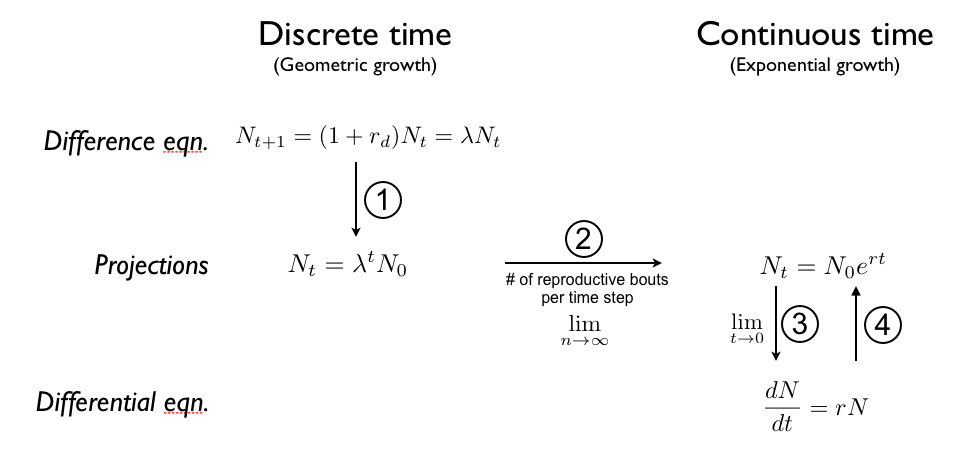
\includegraphics[width=11cm]{figs/EqnConnections.png}
\end{center}

\rule[0.5ex]{\linewidth}{1pt}

\circled{1}
We started with $N_{t+1}=N_t + B + D + I +E$, then substituted $E=I$, $B=bN_t$ and $D=dN_t$, where $b$ and $d$ were per capita rates.
Using $r_d=b-d$ and $\lambda = 1+r_d$, we then simplified down to $N_{t+1} = (1_+r_d)N_t = \lambda N_t$.  Thus, for example,
\begin{equation*}
	N_{t+2}=\lambda N_{t+1}= \lambda (\underbrace{\lambda N_t}_{N_{t+1}}) = \lambda^2 N_t,
\end{equation*}
such that more generally we can write $\boxed{N_t=\lambda^t N_0}$ for any arbitrary $t$ time-steps into the future.

\rule[0.5ex]{\linewidth}{1pt}

\circled{2}
From the discrete to the continuous:
Let's say that in t=1 year an annually reproducing (and dying) population grows by a factor of $\lambda$.  From that one reproductive event we'd have:
\begin{align*}
\text{1 event per time-step:}&\\
	& N_1 = \lambda N_0=(1+r_d)N_0
\end{align*}
Now, if we had 2 reproductive events per year but achieved the same total amount of population growth over the year, we'd write
\begin{align*}
\text{2 events per time-step:}&\\
	& N_1 = \left(1+\tfrac{r_d}{2}\right)^2 N_0
\end{align*}
By extension, if we had an $n$  reproductive events per year but achieved the same total amount of population growth over the year, we'd write:
\begin{align*}
n \text{ events per time-step:}&\\
	& N_1 = \left(1+\tfrac{r_d}{n}\right)^n N_0
\end{align*}
Now, $\lambda$ is nothing more than the discrete population growth factor (how much the population size changed over one year), so let's divide both sides by $N_0$ to isolate $\lambda$:
\begin{align*}
	 \lambda  = & \frac{N_1}{N_0}=\left(1+\tfrac{r_d}{n}\right)^n
\end{align*}
We won't prove it, but by demonstration (see next page):
\begin{equation*}
	\lambda = \lim_{n \to \infty}\left(1+\tfrac{r_d}{n}\right)^n = e^r
\end{equation*}
Therefore, we have
\begin{equation*}
	\boxed{\lambda = (1+r_d) = e^r}
\end{equation*}
and we can relate (convert between) discrete-time and continuous-time population growth:
\begin{equation*}
	\boxed{N_t=N_0 \lambda^t=  N_0 e^{rt}}
\end{equation*}

\rule[0.5ex]{\linewidth}{1pt}
How does Euler's number, $e$, emerge?\\
Let's let $n=1, \; N_0=1, \; r_d=1$\\
The true of $e$ = $exp(1) = 2.71828...$, but we'll estimate it as $\lambda = \tfrac{N_1}{N_0}$ for ever increasing values of $n$:
\begin{align*}
	n=1 \Rightarrow & \frac{N_1}{1}= \left(1+\tfrac{1}{1}\right)^1= 2 \\
	n=2 \Rightarrow & \frac{N_1}{1}= \left(1+\tfrac{1}{2}\right)^2= 2.25 \\
	n=3 \Rightarrow & \frac{N_1}{1}= \left(1+\tfrac{1}{3}\right)^3= 2.30707... \\
	n \to\infty \Rightarrow & \frac{N_1}{1} = \left(1+\tfrac{r_d}{n}\right)^n =  2.71828... = e
\end{align*}
In graphical form:
\begin{center}
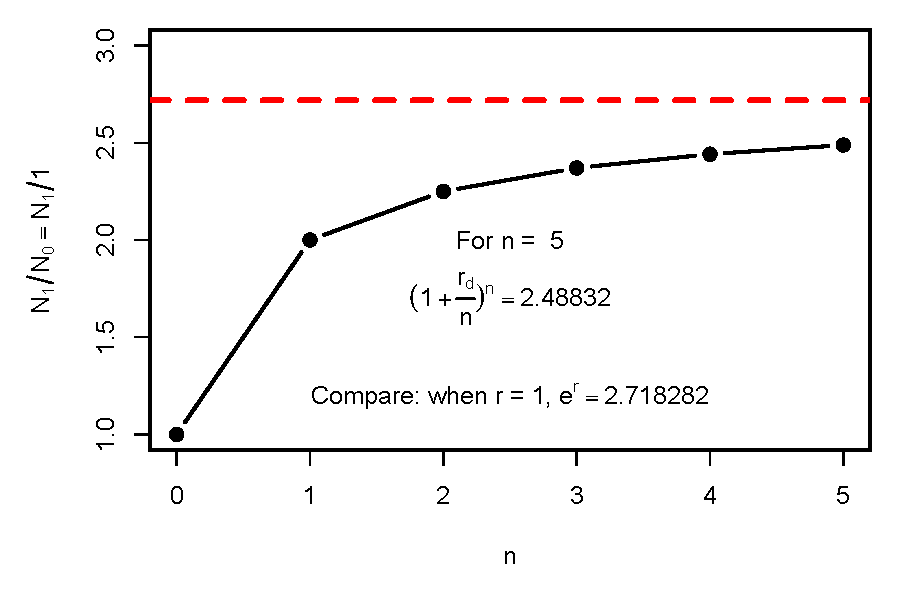
\includegraphics[width=0.45\linewidth]{figs/Rplot1}
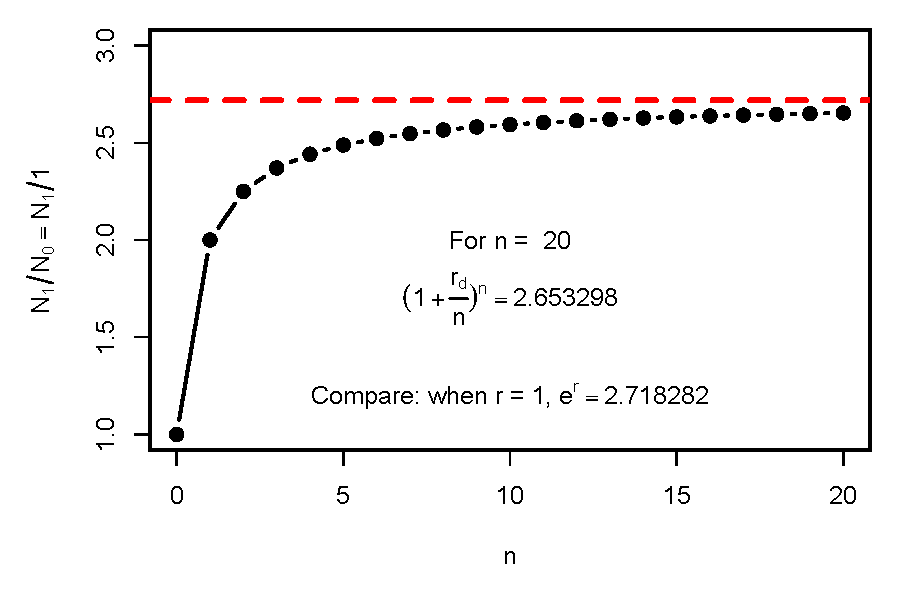
\includegraphics[width=0.45\linewidth]{figs/Rplot2}
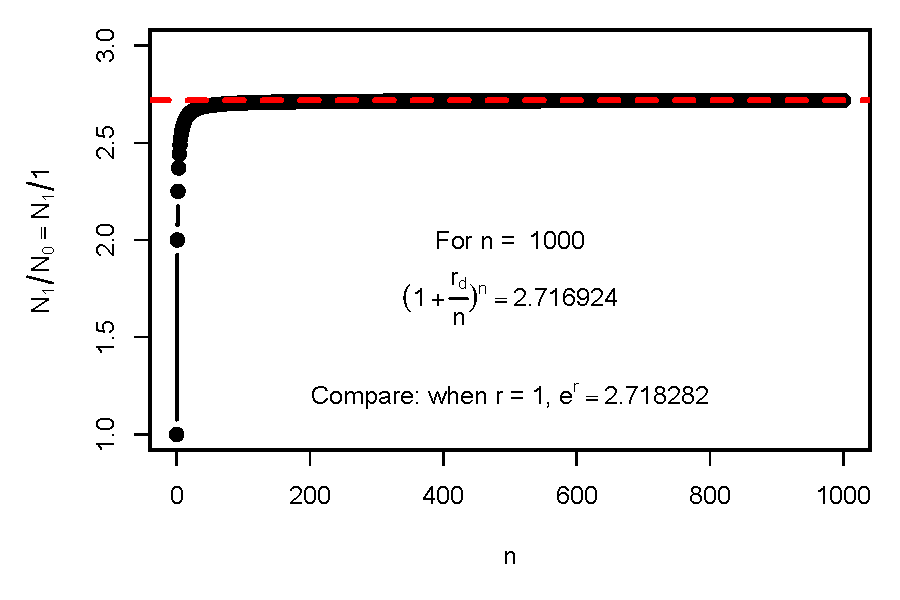
\includegraphics[width=0.6\linewidth]{figs/Rplot3}
\end{center}

\rule[0.5ex]{\linewidth}{1pt}

Defining the natural-log as the `anti-exponential' --- $ln(e^x)=x$ --- we also have:
\begin{equation*}
	ln(\lambda)=ln(1+r_d)=r
\end{equation*}
All three ($\lambda$, $r_d$, and $r$) reflect a \emph{per capita growth rate} for either geometric or exponential growth:
\begin{align*}
	r_d= & b_d-d_d &\text{discrete time}\\
	r=& b-d & \text{continuous time}
\end{align*}

\rule[0.5ex]{\linewidth}{1pt}

\pagebreak

\circled{3}  How to we get instantaneous population-level growth rate from projection equation, $N_0 e^{rt}$?\\ That is, how do we show that:
\begin{equation*}
\lim_{\Delta t \to 0}\left(\frac{\Delta N_t}{\Delta t}\right) = \frac{dN}{dt}
\end{equation*}

Need to take the derivative of $N_0 e^{rt}$ with respect to time $t$.

Use Chain Rule:
\begin{equation*}
\frac{d(XY)}{dt}=\frac{d(X)}{dt}\cdot Y + X \cdot \frac{d(Y)}{dt}
\end{equation*}
(The derivative of a product is the sum of the product of the derivative of each term times the other term.)
Thus:
\begin{equation*}
\frac{d(N_0 \cdot e^{rt})}{dt}=\frac{d(N_0)}{dt}\cdot (e^r)^t + N_0 \cdot \frac{d((e^r)^t)}{dt}
\end{equation*}

Note:\\
Derivative of a constant = 0\\
Derivative of $a^x = ln(a)\cdot a^x$.

Thus:
\begin{align*}
	\frac{d(N_0 e ^{rt})}{dt} & =0 \cdot (e^r)^t + ln(e^r)\cdot (e^r)^t \cdot N_0\\
	&= r \cdot (e^r)^t \cdot N_0\\
	&= r \cdot e^{rt} \cdot N_0 \\
	&= r \cdot N_0 e^{rt} \\
\text{Since } N=N_0 e^{rt} \text{ for any time } t ...&\\
	&=rN=\frac{dN}{dt}
\end{align*}


\rule[0.5ex]{\linewidth}{1pt}

\circled{4} Could also go in opposite direction from $\frac{dN}{dt} \rightarrow N_0 e^{rt}$:
\begin{align*}
&	\frac{dN}{dt}=rN\\
&	\frac{1}{N}\frac{dN}{dt}=r\\
&	\int_0^T \frac{1}{N}\frac{dN}{dt} \; dt = \int_0^T r\; dt \;\;\;\;(\text{Think of T as a constant, and t in dt as a variable})\\
&	\int_0^T \frac{1}{N}\frac{dN}{dt}  = r t \vert_0^T = r \cdot T - r \cdot 0\\
	\text{Using} \; \int \frac{1}{x}\; dx = ln(x)...\\
&	ln(N(T))-ln(N(0))=rT\\
& ln\left( \frac{N(T)}{N(0)}\right) = rT\\
& \frac{N(T)}{N(0)}= e^{rT}\\
& N(T)=N(0)e^{rT}
\end{align*}


\rule[0.5ex]{\linewidth}{1pt}

\end{document}